\documentclass[12pt]{article}

\usepackage{sbc-template}

\usepackage{graphicx,url}

%\usepackage[brazil]{babel}   
\usepackage[latin1]{inputenc}  

\usepackage{amsmath}
\usepackage{amssymb} 
\usepackage{mathtools}

\usepackage{algorithm}
\usepackage[noend]{algpseudocode}

\usepackage{hyperref}
 
\newcommand{\Cfield}{\mathbb{C}}
\newcommand{\Rfield}{\mathbb{R}}

\newcommand{\norm}[1]{\left\lVert#1\right\rVert}

\sloppy

\title{PCS5120 Homework}

\author{Giuliano A. F. Belinassi\inst{1}}


\address{Institute of Mathematics and Statistics (IME) -- University of S�o Paulo
  (USP)\\
  Rua do Mat�o, 1010 -- S�o Paulo -- SP -- Brazil
}

\begin{document} 

\maketitle

%\begin{abstract}

%The Boundary Element Method requires a geometry discretization to execute simulations, 
%and it can be used to analyze the 3D stationary behavior of wave propagation in the soil. 
%Such discretization involves generating two high computational power demanding matrices, 
%and this article demonstrates how Graphical Processing Units (GPU) were used to accelerate 
%this process. In an experiment with 4000 Mesh elements and 1600 Boundary elements, 
%a speedup of 107$\times$ was obtained with a GeForce GTX980. 

%\end{abstract}
     
%\section{Introduction}

In various research fields where numerical linear algebra is required eighter because of 
its facility or inexisence of analytical solutions, can take advantage of packages
such as Lapack or BLAS. One major concern about these libraries is its 
performance, subject discussed in this report. Here we target the routine designed to multiply 
two matrices in single precision floating point (\texttt{SGEMM}).

Althrough implementing a matrix-matrix multiplication seems trivial by its concept, it is 
fairly difficult to provide an efficient code because of various reasons, such as cache usage. 
The use of techniques such as block tiling can yield better results because it improves cache usage, 
but it is important to select the size of the block that results in a best 
overall performance. Such size can be determined empirically.

\section{The database}

We used the database "\textit{SGEMM GPU kernel performance Data Set}" provided by \textit{UCI machine 
learning repository}\footnote{\url{https://archive.ics.uci.edu/ml/datasets/SGEMM+GPU+kernel+performance}}. 
Briefly, it has timings of multiplication of two matrices measured in \textit{ms}, each 
one of size $2048\times2048$, using a combination of $14$ parameters, totalizing $241601$ lines in the database. 
All multiplications were computed using Graphic Processing Units (GPU).

\section{Data analysis}

We used Orange in our analysis. Our first objective was to find the distribuition of the average 
of the four executions per sample to check possible improvements or deterioration of the performance.
For creating a column with the average of four executions, we used the Orange's Feature Constructor. 
Unfortunately, there is no average function implemented here, so we had to calculate such function by 
the definition $\left(\frac{1}{n} \sum{x_i} \right)$. 

Once we had the average column, we plotted the distribution, as illustrated by Figure \ref{fig:freq}. 
Notice that most of the averages concentrate under 200ms, and there are some data around 2400ms. 
Such high timing can be caused by the parameters itself or be an outlier because there were other 
programs running on the computer.

Once we got the distribuition of timings, we focused on what parameters yielded best results. 
Orange's Data Table let us find the combination of parameters because how straightfoward the 
table sorting feature is implemented.

Maybe for pratical reasons, the showed results is enough to provide a setup for an efficient 
implementation, but we can explore the provided data in order to create projections for perhaps
even better timings.

Using the scatterplot tool, we could plot how each parameter impacts the average of timing. 
Analysing such graphics, we could determine that \texttt{MWG}, the tiling line dimension of the matrix, 
is the parameter that mostly impacts 
performance, and such impact is inverse proportional to the timing. So, for a better 
performance, we must minimize the value of \texttt{MWG}. Figure \ref{fig:mwgxavg} illustrates the impact
of this parameter.

Regarding other parameters, we could insert the graphics for each one, but we chose to not do so to 
not extend this report unnecessarily.

\begin{figure}[]
\centering
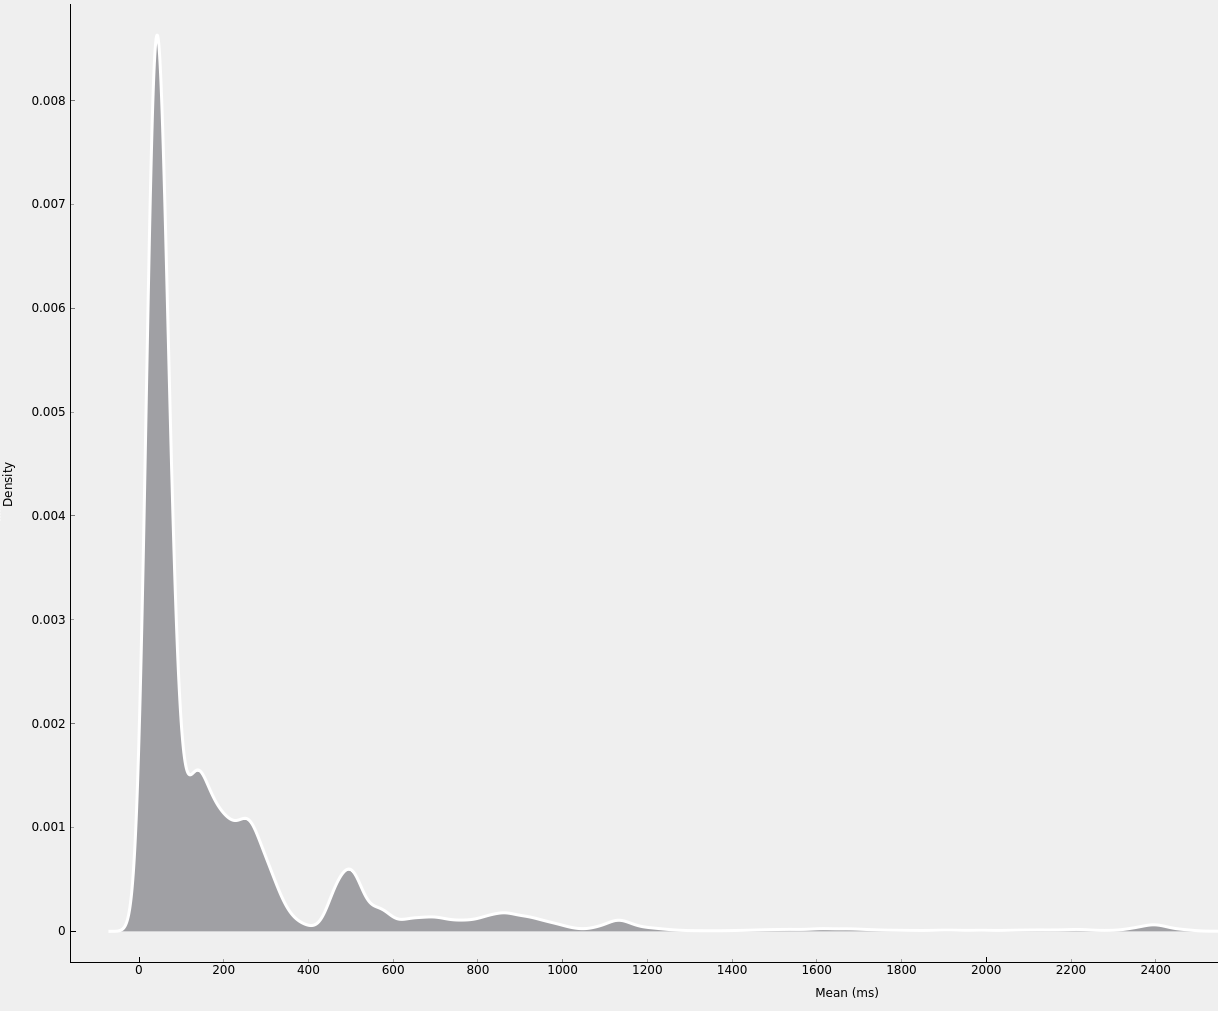
\includegraphics[scale=0.35]{freq.png}
\caption{Distribution of the average of four samples per parameter.}
\label{fig:freq}
\end{figure}

\begin{table}[]
\centering
\caption{Combination of parameters that yielded the 5\# best results}
\label{}
\resizebox{\columnwidth}{!}{%
\begin{tabular}{|l|l|l|l|l|l|l|l|l|l|l|l|l|l|l|}
\hline
MWG & NWG & KWG & MDIMC & NDIMC & MDIMA & NDIMB & KWI & VWM & VWN & STRM & STRN & SA & SB & Mean (ms) \\ \hline
128 & 128 & 16  & 16    & 32    & 32    & 32    & 8   & 2   & 4   & 1    & 0    & 1  & 1  & 13.3175   \\ \hline
128 & 128 & 16  & 16    & 32    & 32    & 32    & 8   & 2   & 4   & 1    & 1    & 1  & 1  & 13.42     \\ \hline
128 & 128 & 16  & 16    & 32    & 32    & 32    & 2   & 2   & 2   & 1    & 1    & 1  & 1  & 13.74     \\ \hline
128 & 128 & 16  & 16    & 32    & 32    & 32    & 8   & 2   & 2   & 1    & 1    & 1  & 1  & 14.4475   \\ \hline
128 & 64  & 16  & 16    & 16    & 16    & 32    & 2   & 2   & 2   & 1    & 0    & 1  & 1  & 14.6325   \\ \hline
\end{tabular}%
}
\end{table}

\begin{figure}[]
\centering
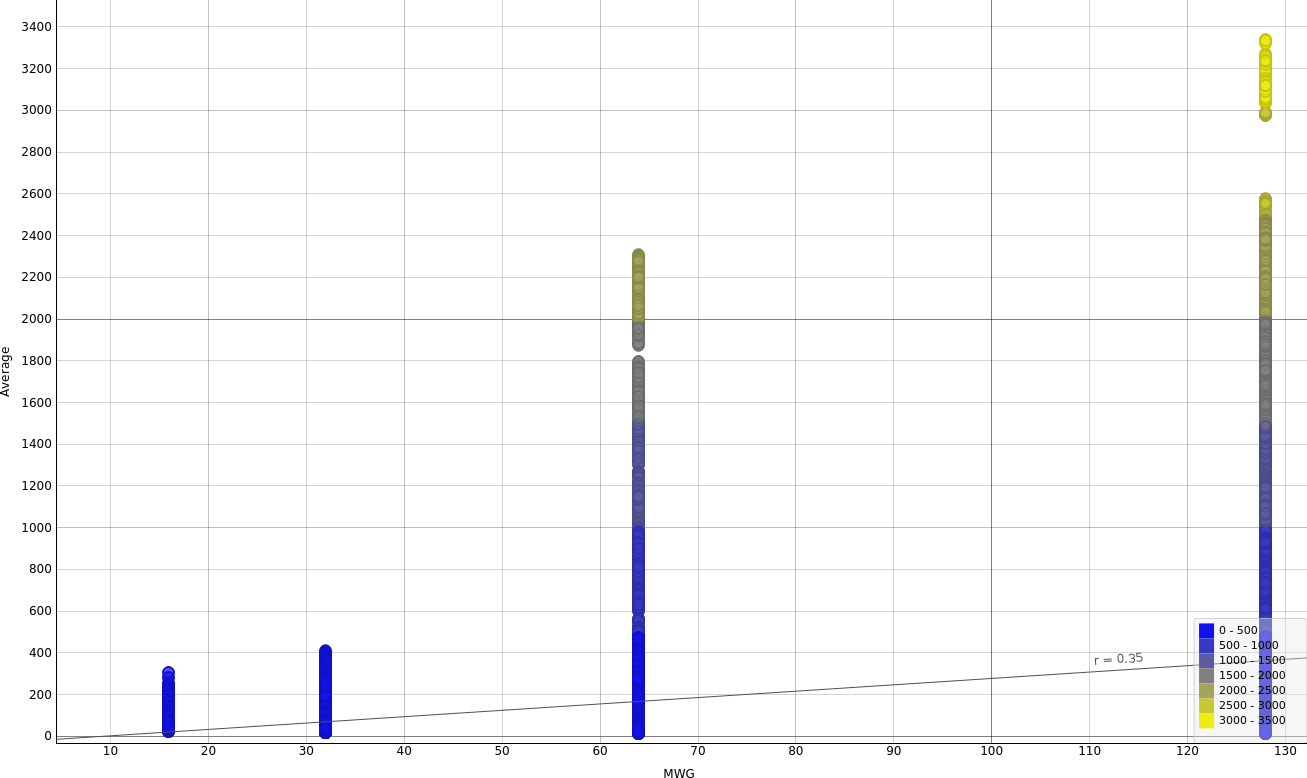
\includegraphics[scale=0.35]{mwgxavg.png}
\caption{Plot of \texttt{MWG} versus Timing Average.}
\label{fig:mwgxavg}
\end{figure}

\section{Conclusions}

Analysing the information in the database in order to extract how the parameters impact 
the overall performance of the routine can aid the development of increasingly efficient 
numerical libraries, and such analysis was made possible by Orange in a visually intuitivelly 
manner. There was no need to write extensive code to prepare the data for being processed, 
nor to plot graphics.

On the other hand, Orange is not a fairly efficient tool performance-wise. For the database 
selected, it used around 12Gb of memory just for loading it, and every step took very long 
to compute and display any result. The use of more efficient data structures and parallel 
computing may address these issues. 

%The current implemented code have limitations. First, there is no logic to construct both $H$ and $G$ by blocks to create several 
%GPU kernels. Second, there is also no logic to compute both $\texttt{Ghmatecd\_Nonsingd}$ and $\texttt{Ghmatecd\_Sing\_de}$ in 
%parallel with respect to each other. The usage of GPUs in the singular case can also be analyzed.


%\begin{figure}[ht]
%\centering
%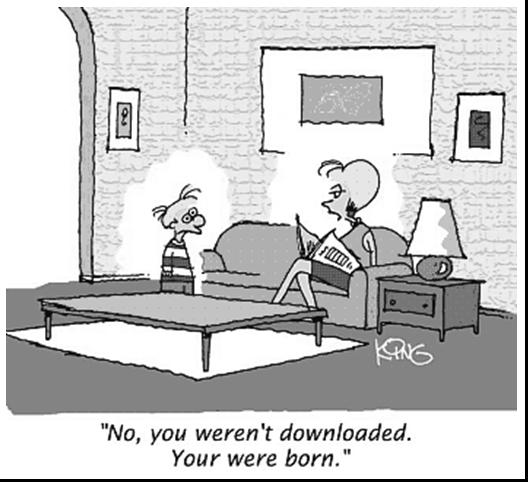
\includegraphics[width=.5\textwidth]{fig1.jpg}
%\caption{A typical figure}
%\label{fig:exampleFig1}
%\end{figure}
%
%\begin{figure}[ht]
%\centering
%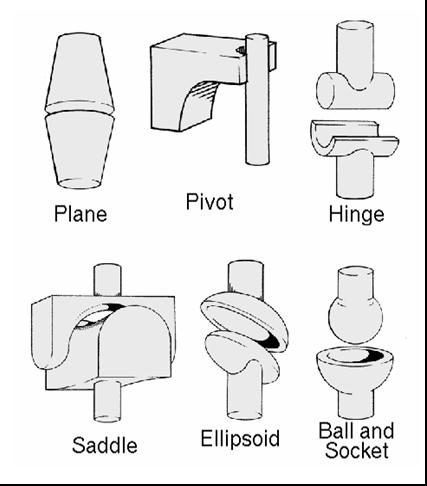
\includegraphics[width=.3\textwidth]{fig2.jpg}
%\caption{This figure is an example of a figure caption taking more than one
%  line and justified considering margins mentioned in Section~\ref{sec:figs}.}
%\label{fig:exampleFig2}
%\end{figure}


\bibliographystyle{sbc}
\bibliography{sbc-template}

\end{document}
\grid
